% !TeX root = ../../main.tex
% Add the above to each chapter to make compiling the PDF easier in some editors.

\section{Generalization Over Domains} \label{ord:ch5:sec2_generalization_image_domains}
% RE-1467
% Motivation - get insights of the performance on other domains (anomaly and industrial)
The ability of methods to generalize well may be crucial to their success in application.
For \gls{dl} methods in general the generalization capability is mostly based on the dataset used for training.
The \gls{dextr} and \gls{iog} method are trained on a combination of PASCAL \gls{voc} and COCO.
These datasets mostly cover general objects and do not contain images from special domains.
In order to examine the method's generalization capabilities, they are evaluated over different domains and datasets.
First, the generalization capabilities of the four benchmark methods are evaluated over image domains from the benchmark study.
Thereby, the performance of $ IoU $ and $ time $ are examined.
Second, simulations are used to evaluate the $ IoU $ of the \gls{dextr} and \gls{iog} method on various datasets.

\subsection{Generalization Over Domains}
% Each method is evaluated over the four domains
In the following it is evaluated how well the four benchmark methods generalize over the four image domains: $ standard $, $ urban $, $ industrial $, and $ anomaly $.
Thereby, the evaluation of the generalization capabilities is twofold based on the $ IoU $ and $ time $.

% IoU
\subsubsection{IoU}
The generalization over the accuracy measured by the $ IoU $ is examined.
The accuracy per method and domain is visualized in Figure \ref{fig:ch5:sec2:methods_over_domain_iou}.

\begin{figure}[h!]
	\centering
	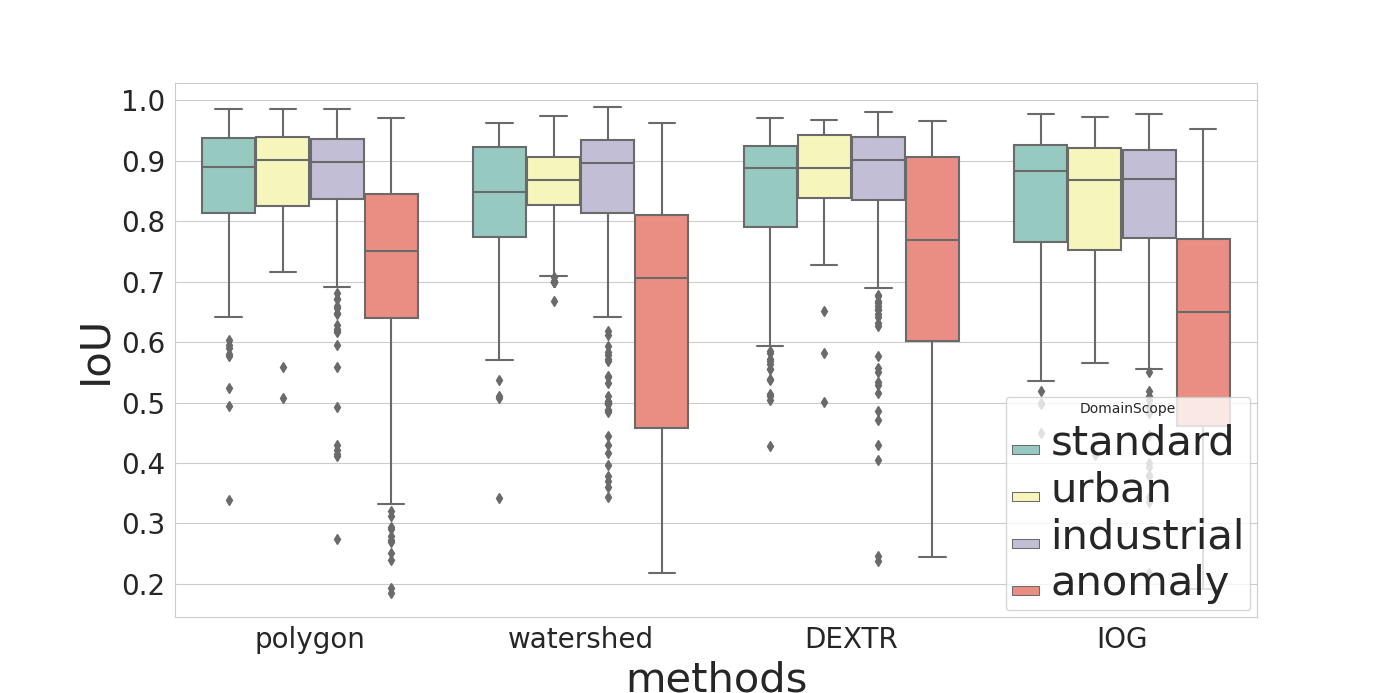
\includegraphics[width=\textwidth]{figures/chap52_iou_methods_over_domains_boxplot.png}
	\caption [Box plots of image domains and methods on  $ IoU $]{
		Box plots of $ IoU $ based on the image domains and benchmark methods.
		The $ IoU $ for the domain $ anomaly $ differs strongly for all methods, which can be explained by the different nature of this domain.
		It seems, that for the other domains all methods perform on a approximately similar level.
	}\label{fig:ch5:sec2:methods_over_domain_iou}
\end{figure}

% Performance of Anomaly
It is immediately noticeable that the \gls{iou} in the domain $ anomaly $ is significantly worse for each method.
This is reasonable due to the different nature of the annotations from this domain.
It was experienced in the review of the user annotations, that for the domain $ anomaly $ the users often have a varying understanding what belongs to the anomaly and what should be labeled.
These ambiguities create room for misinterpretations of the anomaly, which in turn affects the $ IoU $.
However, it may be noted that the \gls{dextr} method performs best on the domain $ anomaly $ most probably due to the strong and direct type of guidance provided by the extreme points.

% Performance of , urban, and 
Further, the four methods deliver comparatively similar results on the three other image domains $ standard $, $ urban $, and $ industrial $.
Thereby, the Kruskal-Wallis test is applied with the $ H_{0} $ already excluding the domain $ anomaly $, because it already can be seen in Figure \ref{fig:ch5:sec2:methods_over_domain_iou}, that $ IoU_{anomaly} $ strongly deviates.
The details of the test are presented in Table \ref{tab:ch5:tests_on_methods}.
%Only for the polygon method $ H_{0} $ is rejected at $ \alpha = 1\% $, while for the other methods $ H_{0} $ is narrowly accepted.
However, it is important to highlight, that this results strongly depends on the chosen significance level $ \alpha $.
The close decisions diminishes the significance of the statistical analysis and state that there is no clear decision as here.

However, it may be said that for the methods watershed, \gls{dextr}, and \gls{iog} the accuracy does not differs strongly over the three image domains $ standard $, $ urban $, and $ industrial $.
From this it can be concluded that these methods sufficiently generalize over different domains.
It is notable, that the \gls{dextr} and \gls{iog} method do not necessarily perform better on the domain $ standard $, even though they have been explicitly trained with this type of images. 
This also confirms the results from \cite{Man18-DEXTR} and \cite{Zha20-IOG}, which emphasize the performance of their methods across domains.
Although in general, an improvement of performance could be still possible if the model would be trained on the same type of images that are used for the evaluation.
This is strongly assumed, but not pursued further within the scope of this work.

\begin{table}[h!]
	\centering
	\begin{tabular}{l|p{25mm} p{25mm} p{25mm} p{25mm}}
		\toprule 		
		& \centering $ Polygon $	& \centering $ Watershed $ 	& \centering $ DEXTR $ 	& \multicolumn{1}{c}{$ IOG $}	\\
		\midrule
		$ n_{annots} $	& \centering 81				& \centering 98				& \centering 87			& \multicolumn{1}{c}{81}  		\\
		$ H_{0} $		& \multicolumn{4}{c}{$ med \left( IoU_{standard} \right) = med \left( IoU_{urban} \right) = med \left( IoU_{industrial} \right)$}  \\  
		$ H_{A} $		& \multicolumn{4}{c}{$ H_{0} = false $}  \\ 	
		$ \alpha $		& \centering $ 1\% $ 		& \centering $ 1\% $ 		& \centering $ 1\% $ 	& \multicolumn{1}{c}{$ 1\% $} 	\\ 	
		Statistic		& \centering 12.5154		& \centering 6.3355      	& \centering 9.0211		& \multicolumn{1}{c}{1.3372}  	\\ 
		$ \textnormal{\textit{p-value}} $
		& \centering 0.0019			& \centering 0.0421 		& \centering 0.0109		& \multicolumn{1}{c}{0.5124}	\\
		$ H_{0} $		& \centering rejected 		& \centering accepted	  	& \centering accepted 	& \multicolumn{1}{c}{accepted}  \\ 										
		\bottomrule
	\end{tabular}
	\caption[Kruskal-Wallis test performed on methods over domains]{
		For each benchmark method the Kruskal-Wallis test is applied to compare the $ IoU $ over the benchmark domains $ standard $, $ urban $, and $ industrial $.
		The domain $ anomaly $ is not included in this test, because it already can be seen in Figure \ref{fig:ch5:sec2:methods_over_domain_iou}, that the $ IoU $ differs for this domain.
		All tests are performed on the same $ H_{0} $ and $ H_{A} $.
		The number of annotations $ n_{annots} $ varies, because for each method the Kruskal-Wallis test requires the same size for the factors.
	}\label{tab:ch5:tests_on_methods}
\end{table}

% Time
\subsubsection{Time}
Further, the method's generalization capabilities are evaluated based on $ time $.
An overview of the annotation time per method and domain is provided by the box plots in Figure \ref{fig:ch5:sec2:methods_over_domain_time}.
% For Polygon and Watershed the domains  and urban require much time while the  and Anomaly are fast.
It is easy to see that more time is spent on the domains $ standard $ and $ urban $ than on the domains $ industrial $ and $ anomaly $.
This probably follows from the fact that the objects from domains $ standard $ and $ urban $ are more complicated and therefore require more annotation time.
% This behaviour may also be observed for DEXTR and IOG but not this extreme -> good generalization.
This behavior is extreme for watershed method and decrease continuously across the methods polygon, \Gls{iog}, and \gls{dextr}.

% Noteable in general is the larger annotation time for polygon and watershed.
In general, this demonstrates that the longer annotation time of polygon and watershed spans across the image domains.
It can be said that the \gls{dextr} and \gls{iog} method also generalize well based on the annotation time, since the values for $ time $ are in a similar range over the image domains.

\begin{figure}[h!]
	\centering
	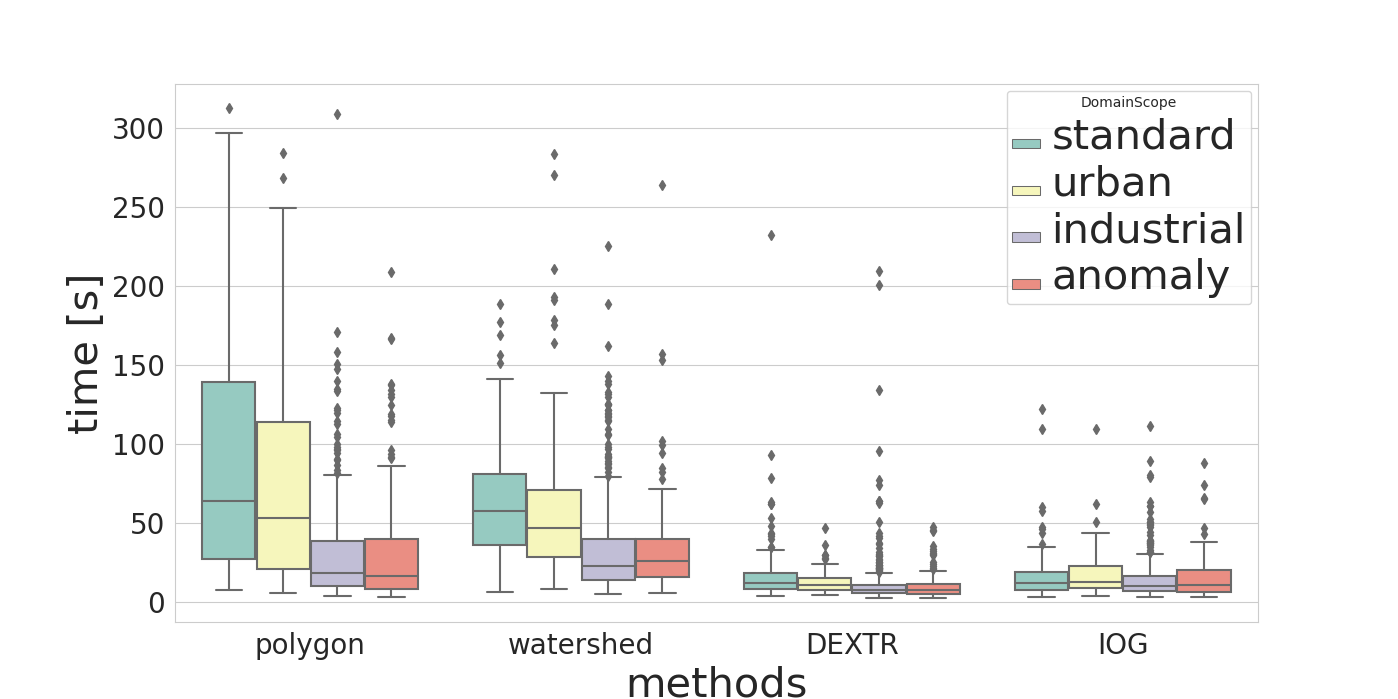
\includegraphics[width=\textwidth]{figures/chap52_time_methods_over_domains_boxplot.png}
	\caption[Box plots of image domains and methods on  $ time $]{
		Box plots of $ time $ based on the image domains and benchmark methods.
		For the domains $ standard $ and $ urban $ the $ time $ is clearly higher, than for the other domains.
		This is extreme for the methods polygon and watershed.
		A difference may be noted for \gls{dextr} and \gls{iog} as well, but in general the generalization capabilities are sufficient.	
	} \label{fig:ch5:sec2:methods_over_domain_time}
\end{figure}

\begin{comment}
% Grouped by dataset with methods as factors
\subsection{Generalization Of Domains Over Methods} \label{ord:ch5:sec2:subsec1}
% For all methods - Kruskal-Wallis test (or even ANOVA) for the domains as factors
The sample is split up by the benchmark domains, introduced in Section \ref{ord:ch4:sec4}, and evaluated for each domain.
For this the Kruskal-Wallis test is applied to each split with the four benchmark methods as factors.
Due to the split by the four domains and the requirement of the same factor size by the Kruskal-Wallis test, the number of samples per factor is reduced to $n_{annots}$ in this test setup.
The details and results of the tests is shown in Table \ref{tab:ch5:tests_on_domains} and the corresponding box plot of illustrated in Figure \ref{fig:ch5:sec2:domains_box_plot}.

For the domains $ standard $ and $ urban $, which are similar to PASCAL \gls{voc} and COCO, $ H_{0} $ is accepted and the benchmark methods do not differ significantly.
In contrast, for the domains $ industrial $ and $ anomaly $ $ H_{0} $ is rejected and $ H_{A} $ accepted. Therefore, there is some significant difference between the benchmark methods.
\begin{table}[h!]
	\centering
	\begin{tabular}{l|p{25mm} p{25mm} p{25mm} p{25mm}}
		\toprule 		
								& \centering $ standard $	& \centering $ urban $  		& \centering $ industrial $ & \multicolumn{1}{c}{$ anomaly $} \\
		\midrule
		$ n_{annots} $			& \centering 105				& \centering 81				& \centering 351 			& \multicolumn{1}{c}{82}  \\
		$ H_{0} $				& \multicolumn{4}{c}{$ med \left( IoU_{polygon} \right) = med \left( IoU_{watershed} \right) = med \left( IoU_{IOG} \right) = med \left( IoU_{DEXTR} \right) $}  \\  
		$ H_{A} $		 		& \multicolumn{4}{c}{$ H_{0} = false $}  \\ 	
		$ \alpha $		 		& \centering $ 1\% $ 		& \centering $ 1\% $ 		  	& \centering $ 1\% $ 		& \multicolumn{1}{c}{$ 1\% $} 	\\ 	
		Statistic		 		& \centering 4.8254			& \centering 12.692	      		& \centering 30.3888			& \multicolumn{1}{c}{14.4029}  	\\ 
		$ \textnormal{\textit{p-value}} $
								& \centering 0.1850			& 0.0054 	& \centering $ 1.1 \cdot 10^{-6}$		& \multicolumn{1}{c}{0.0015}	\\
		$ H_{0} $		  		& \centering accepted 		& \centering rejected	  		& \centering rejected 		& \multicolumn{1}{c}{rejected}  \\ 										
		\bottomrule
	\end{tabular}
	\caption[Kruskal-Wallis tests over domains]{
		Four Kruskal-Wallis tests are applied for the domain scopes $ standard $, $ urban $, $ industrial $, and $ anomoaly $.
		The four benchmark methods are used as factors for each test.
		All tests are performed on the same $ H_{0} $, $ H_{A} $ and the same sample $X_{raw}$.
	}\label{tab:ch5:tests_on_domains}
\end{table}

The post analysis is performed by the DSCF test \cite{CF91-dscf}, which determines the factor, that differs significantly in the domains $ industrial $ and $ anomaly $.
As a result, for the domain $ standard $ only the \gls{iog} method gave evidence for a statistical significant decrease in performance.
In the domain $ anomaly $ two groups are formed, \gls{dextr} and Polygon achieve a significantly higher $ IoU $ than \gls{dextr} and Watershed.
Inside these two groups no significant difference occurs.
% Box plot with 16 "cols" - 4 methods x 4 domains
\begin{figure}
	\centering
	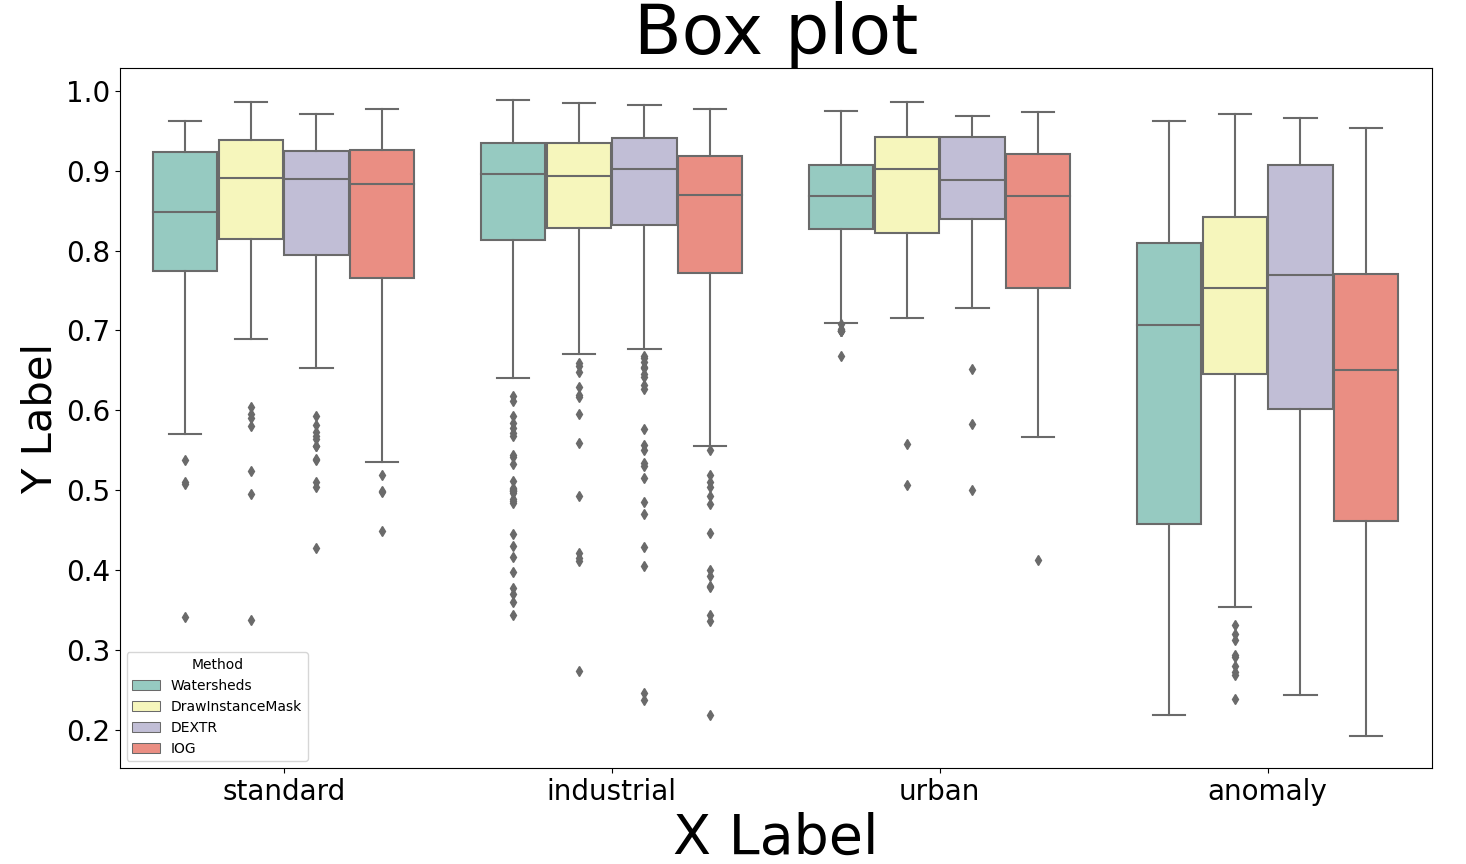
\includegraphics[width=0.9\textwidth]{figures/chap52_boxplot.png}
	\caption[Box plot IoU per domain and method]{
		Box plot of the $ IoU $ per image domain and benchmark method.
		In the domain $ anomaly $ all methods perform worse compared to the other domain, due to the special characteristics of this domain.
		For the domain $ anomaly $, $ med \left( IoU_{IOG} \right) $ is significantly lower, than for the other methods.
		The domains $ industrial $ and $ urban $ do not evidence a statistically significant difference between the methods.
	} \label{fig:ch5:sec2:domains_box_plot}
\end{figure}

Further, it was detected, that the domains $ urban $, $ industrial $, and $ anomaly $ do not differ significantly in their median value of the $ IoU $.
Only the domain scope $ anomaly $ differs greatly, which is reasonable due to the clearly different types of images.
It was experienced in the review of the user annotations, that the users often have a varying understanding what belongs to the anomaly, which should be labeled.
This ranges from different to misinterpretations, which also in an explanation for the general lower $ IoU $ in this domain.
The good performance of the polygon and \gls{dextr} method in the domain $ anomaly $ most probably is caused by the strong and direct type of guidance provided by the user interaction.

In conclusion it may be stated, that the examined benchmark methods mostly do not significantly vary over common domains, excluding the domain $ anomaly $.
Only for the \gls{iog} method did not generalize as well as the other methods on the domain $ standard $.
some comment
\end{comment}

\subsection{Generalization Over Datasets} \label{ord:ch5:sec2:subsec2}

In order to further evaluate the \gls{dextr} and \gls{iog} method, simulations are applied on various datasets from various domains.
To continue the evaluation of the generalization capabilities datasets from different domains are used.
First, the performance of the initial prediction over multiple datasets is presented, while later the refinement results are examined. 

\subsubsection{Initial Prediction}

% Define simulation settings
The different simulation setups from the original \gls{dextr} \cite{Man18-DEXTR} and \gls{iog} \cite{Zha20-IOG} have been implemented in HDevelop and unified to allow a fair comparison. 
Thereby, the \gls{gt} is used to simulate the user clicks on fore- and background to create the required model input.
It has to be highlighted, that this simulation setup only contains little deviation or randomness, similar to the original simulation setup from \gls{dextr} and \gls{iog}.
As a result, the simulated user clicks are almost perfect.
More realistic user clicks can be simulated by the inclusion of random deviation, which is presented in Subsection \ref{ord:ch5:sec3:subsec3}.

The performance of the \gls{dextr} and \gls{iog} method on various datasets is shown in Table \ref{tab:ch5:tests_on_datasets}.
It can be seen, that in general the \gls{iog} method performs best, except for the benchmark dataset, where \gls{dextr} achieves a higher \gls{miou}.
The superiority in the simulation of \gls{dextr} on this data set is consistent with the results from the real users from the benchmark study.

\begin{table}[h!]
	\centering
	\begin{tabular}{l|c c}
		\toprule 		
										& \multicolumn{2}{c}{mIoU}\\
										&  DEXTR 	& IOG		\\
		\midrule
		PASCAL (VP \cmark)				& 0.9103 	& 0.9251	\\
		PASCAL (VP \xmark)				& 0.7805	& 0.8086	\\
		Benchmark Dataset				& 0.8394 	& 0.8201	\\
		MVTec D2S						& 0.9297	& 0.9342	\\
		Segmentation and Counting		& 0.8280	& 0.8797 	\\							
		\bottomrule
	\end{tabular}
	\caption[Generalization of IOG and DEXTR]{
		The \gls{dextr} and \gls{iog} method are applied on multiple datasets to evaluate their performance over several domains.
		For the PASCAL \gls{voc} dataset the performance is measured with (\gls{vp} \cmark) and without (\gls{vp} \xmark) the application of the \gls{vp}.
	}\label{tab:ch5:tests_on_datasets}
\end{table}

The difference in accuracy for the PASCAL \gls{voc} dataset \cite{Eve20-PascalVOC} with and without the application of \gls{vp} is especially interesting.
The meaningfulness of \gls{vp} is already addressed in Subsection \ref{ord:ch2:sec2} and their effect can be observed in Table \ref{tab:ch5:tests_on_datasets}.
For \gls{dextr} the difference in \gls{miou} is around $ 0.13 $ and for \gls{iog} almost $ 0.12 $.
This represents a significant decrease in accuracy, which raises doubts how expressive the results with the applications of \gls{vp} are.
Especially problematic is that the \gls{vp} are located at the edge of an object, which is generally difficult to predict.
As a consequence, it may not be recognized if a model's weakness is the prediction of the edges.
Therefore, the use of \gls{vp} may lead to unrealistic expectations on the method's accuracy, which are mostly not achievable in real world application.
The presentation of the performance without \gls{vp} would lead to more transparency and awareness of this characteristic.

\subsubsection{Refinement Prediction}

% Show a table displaying the performance for various refinement clicks on multiple dataset
Last, the performance of the method with the application of refinement is evaluated on different datasets.
Thereby, for each method five refinement clicks were simulated.
For the \gls{iog} method, the refinement clicks can be on the fore- and background, while the \gls{dextr} method only allows refinement clicks on the border.
The refinement clicks are simulated using the \gls{gt}.
A click is set on the region where the previous prediction fails.

\begin{table}[h!]
	\centering
	\resizebox{\textwidth}{!}{
	\begin{tabular}{l l|c c c c c c}
		\toprule
				&						& \multicolumn{6}{c}{mIoU} \\
				& {$ n_{\textnormal{\textit{refine clicks}}} $} 
										& 0			& 1			& 2			& 3 		& 4 		& 5			\\
		\midrule
		DEXTR 	& PASCAL (VP \cmark)	& 0.9103	& 0.9119	& 0.9054	& 0.8986 	& 0.8916	& 0.8863	\\
			 	& PASCAL (VP \xmark)	& 0.7805	& 0.7894 	& 0.7893	& 0.7871 	& 0.7833	& 0.7807	\\
				& Benchmark				& 0.8394	& 0.8522 	& 0.8513	& 0.8504 	& 0.8512	& 0.8492	\\
				& MVTec D2S				& 0.9297	& 0.9416 	& 0.9436	& 0.9437 	& 0.9419	& 0.9397	\\
		\midrule
		IOG 	& PASCAL (VP \cmark)	& 0.9251	& 0.9359	& 0.9402	& 0.9436 	& 0.9449	& 0.9459	\\
				& PASCAL (VP \xmark)	& 0.8086	& 0.8184	& 0.8259	& 0.8313 	& 0.8351	& 0.8381	\\
				& Benchmark				& 0.8219	& 0.8396 	& 0.8508	& 0.8601	& 0.8669	& 0.8715	\\
				& MVTec D2S				& 0.9343	& 0.9358 	& 0.9424	& 0.9468 	& 0.9499	& 0.9523	\\
		\bottomrule
	\end{tabular}}
	\caption[Generalization of IOG and DEXTR refinement]{
		Performance of the \gls{dextr} and \gls{iog} method for different number of refinement clicks.
		At $ n_{\textnormal{\textit{refine clicks}}} = 0 $, no refinement click is set, which is equivalent to the initial prediction.
	}\label{tab:ch5:tests_on_refinement_datasets}
\end{table}

In Table \ref{tab:ch5:tests_on_refinement_datasets} the performance of the methods is presented for various refinement clicks.
For \gls{dextr} mostly only the first refinement clicks leads to a improvement, while the further clicks keep or decrease the \gls{miou}.
In contrast, the \gls{iog} method is able to profit from each refinement click and increase the \gls{miou}. 
From the ninth click, the improvement stagnates or worsens slightly as shown in Table \ref{tab:appendix_refinementclicks}.
It can be stated, that refinement process generalizes well and performs expected over several domains.
